% Chapter Template

\chapter{内存分离} % Main chapter title

\label{Chapter2} % Change X to a consecutive number; for referencing this chapter elsewhere, use \ref{ChapterX}

% 论点:
% 1. 阐述内存分离技术的重要意义
% 2. 阐述内存分离技术目前的研究现状,相当于related work
% 3. 以INFINISWAP为例来最先进内存分离技术。
% 4. 自己的启发性思考
%

内存资源在数据中心中相对昂贵而且稀少的资源,如何利用好内存资源一直都是学术界以及工业界的一个研究重点。
其中,一个主要研究方向是内存分离(memory disaggregation)。
将内存资源从一体化服务器(monolithic server)中解耦出来,服务器上的应用能同时访问“本地”的和“远端”的内存,看上去就像是访问一块内存一样,这样的技术被称为内存分离(memory disaggregation)。
通过内存分离,应用程序能使用到更多的内存资源,也减少了内存利用率不高而导致的资源、能源浪费的情况。
本章节将主要通过介绍INFINISWAP系统,来介绍内存分离的一个具体实现并通过这个具体实现来理解。

在本章的开始,我们先介绍内存分离技术的研究背景,从而了解数据中心对内存资源的需求和内存分离技术出现的缘由。
再分类地说明内存分离的研究现状,介绍内存分离不同的研究方向以及其对应的技术。
接着,我们着重介绍再内存分离技术领域比较先进的INFINISWAP系统\cite{gu2017efficient}。
最后我们对内存分离技术做一个总结,并提出一些我们的问题和思考。

%----------------------------------------------------------------------------------------
%	SECTION 1
%----------------------------------------------------------------------------------------

\section{背景介绍}

\subsection{问题来源}
内存不足的现象是自内存设备出现以来就已经存在的问题。
在过去,解决内存不足问题的目标仅仅是说让程序在内存不足的时候也能正确运行,因此产生了虚拟内存(virtual memory)、换页(paging)等技术来缓解内存不足的状况,本质是通过硬盘来暂存内存数据,这样的方法虽然解决了内存不足的问题,但性能却很差。

现在,虽然单机上的内存的容量已经增大了很多,但内存不足的情况依旧存在。
因为应用程序对于内存的需求也越来越大了,而换页的性能很差,并不能满足应用的需求。
除了内存不足的问题,新的问题也逐渐涌现。
并不是所有的应用程序都会都将本机的所有内存全部使用,因此出现内存过剩的资源浪费问题。

内存不足与内存过剩是一对矛盾,却又会同时出现,这展现出的是内存使用的不均衡性。
其根本原因是传统的一体化服务器的架构给内存的部署、分配和使用所带来的限制。
一方面,单机上内存资源在服务器部署之后就已经基本上是确定不变的了,服务器部署运行之后再去拓展内存资源是一件麻烦而且成本大的事情。
另一方面,单台服务器所能支持的最大内存是有限,这必然不能满足应用程序日益增长的内存需要。

\subsection{研究意义}
首先,为了说明内存不足而导致换页的不利影响,有相关研究人员做了一些测试\cite{gu2017efficient}。
他们选择了三种不同的内存应用程序进行测试:(i)运行在VoltDB内存数据库上的TPC-C基准测试程序;
(ii)运行在Memcached键值仓储中的模拟facebook工作负载的程序;
(iii)运行在PowerGraph的TunkRank算法,使用的数据集是Twitter。

\begin{figure}
\centering
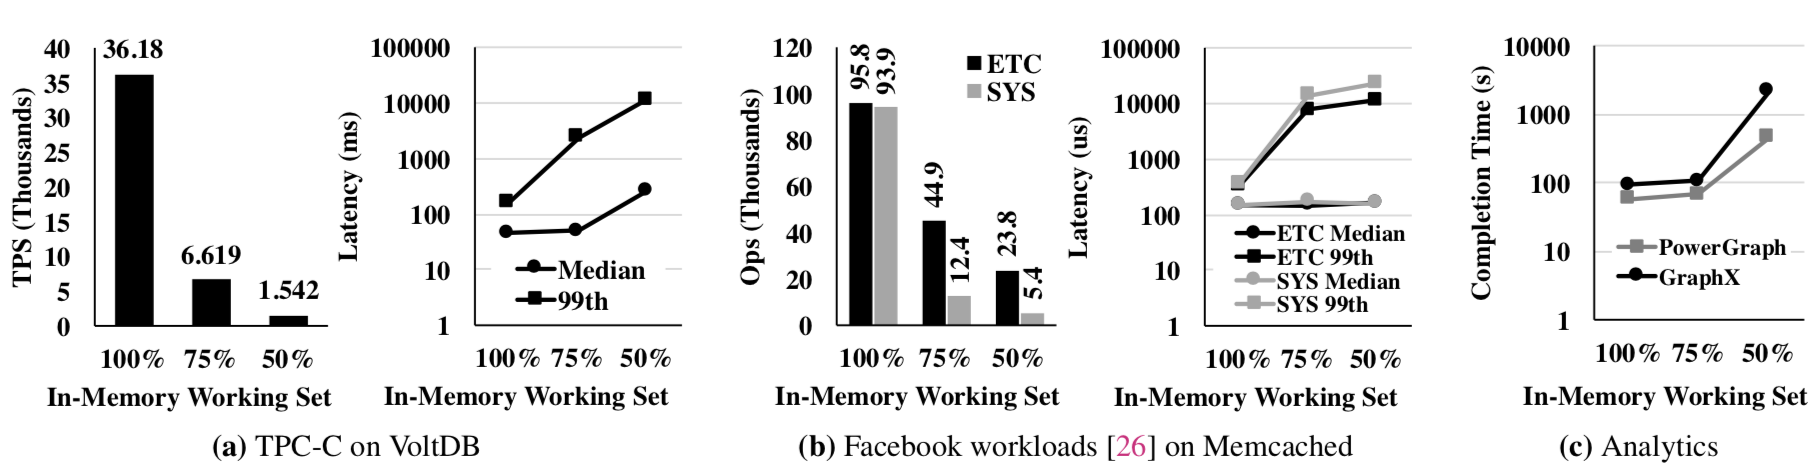
\includegraphics[scale=0.45]{Figures/memory/memory_motivation1.png}
\decoRule
\caption{在不同内存容量下应用程序的性能\cite{gu2017efficient}。}
\label{fig:memory_motivation1}
\end{figure}

为了避免由外部因素造成的性能影响,测试只关注应用程序在单机下的性能(图~\ref{fig:memory_motivation1})。
结果显示由于内存不足所导致的换页确实对应用程序产生重大的、非线性的、急速下降的性能影响。
另外,换页会导致非常明显的尾延迟现象。
以上的现象都表明,内存不足是一个非常重要的问题,进行内存分离的研究是十分有必要的。

\begin{figure}
\centering
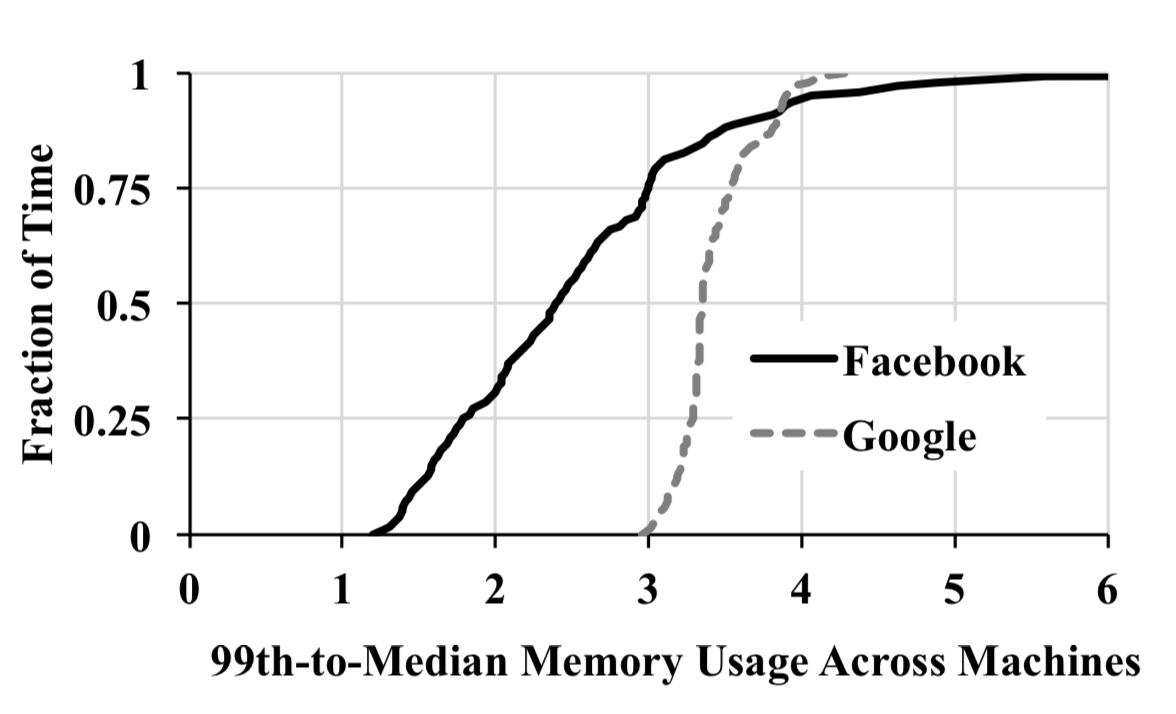
\includegraphics[scale=0.6]{Figures/memory/memory_motivation2.png}
\decoRule
\caption{Facebook和Google的两个机器集群中存在的内存使用不均衡现象\cite{gu2017efficient}。}
\label{fig:memory_motivation2}
\end{figure}

其次,不同机器中的内存使用也存在着不均衡的现象,这将导致资源浪费。
有相关的研究人员统计了Google和Facebook的两个实际运行的集群中机器内存使用情况的一些数据(图~\ref{fig:memory_motivation2})。
通过记录和计算10秒内前99\%的机器的平均内存使用率与所有机器平均使用率的比值,来表示内存使用的不均衡性。
结果显示,集群中有超过一半的内存因资源利用不均衡而导致其未被使用到的。
这样的资源利用不均衡也验证了我们的说法。


%----------------------------------------------------------------------------------------
%	SECTION 2
%----------------------------------------------------------------------------------------

\section{当前内存分离技术的研究现状}

很长一段时间以来,数据中心都在使用着一体化服务器的架构,使得大多数内存分离技术都是基于这种架构去设计并实现的,如分布式共享内存(distributed share memory)技术和远程换页(remote paging)技术。
这些方法考虑的是易用性、可行性,不需要对现有服务器架构设计进行太大的修改。

内存分离技术有多种不同维度的划分方法。
LegoOS\cite{shan2018legoos}的研究人员按照软硬件的划分将内存分离技术分成两大类,一类是硬件辅助的内存分离技术,指的是设计一些专用的小硬件来辅助和加速内存分离;
另一类是纯软件实现的内存分离技术,只需要现有的硬件设备来实现内存分离。
而INFINISWAP的研究人员则是按照实现方法划分,将内存分离技术主要分为远程内存换页技术(Remote Memory Paging)和分布式共享内存(Distributed Shared Memory)两大类。

我们认为INFINISWAP的技术划分思路更加有实际意义,但我们要进行一定的补充,我们认为内存分离技术可以分为如下几类:

\begin{itemize}
\item \textbf{分布式应用程序。}
应用开发者需要显示地根据多台服务器编程,让多台服务器共同协作。
分布式应用程序的出现一开始是因为单台服务器的计算能力有限,需要多台服务器去提升应用的计算速度。
但现在也可以用来解决单台服务器上内存资源不足的问题。
这种方法的优点是应用程序的性能能够被充分优化;缺点是编程复杂、开发困难。

\item \textbf{新硬件辅助内存分离。}
在现有的一体化服务器架构的基础上,通过增加一些小的新硬件来使能与加速对远端机器的访问。
这种方法的优点是速度快,不需要对现有的服务器硬件架构做很大的修改;缺点是新硬件的生产和部署不太实际。

\item \textbf{远程内存换页技术和分布式共享内存技术。}
远程换页技术和分布式共享内存技术都是向应用程序做了隐藏,使应用可以在“不知情”的状况下使用本地和远端内存。
这些方法的优点是不需要修改应用程序,具有很好的通用性与实际性;缺点是性能会比较差。

\item \textbf{新的服务器架构。}
最近,有一些研究提出了更大胆更激进的资源分离的做法,抛弃现有的一体化服务器的架构,将各类硬件资源彻底分离。
其从根本上解决了一体化服务器的弊端,但要真正投入到生产使用还需要很长的时间。

\end{itemize}


%----------------------------------------------------------------------------------------
%	SECTION 3
%----------------------------------------------------------------------------------------

\section{案例:基于RDMA高速网络的内存分离技术——INFINISWAP}

INFINISWAP是针对RDMA高速网络设计的一个远程换页系统,通过将集群中每台机器的交换分区划分成大块去管理,适时地去收集机器中未使用的内存,并把这些内存暴露给应用程序使用。
整个过程对于应用程序来说是透明不可见的,因而应用程序不需要做任何修改。
在接下来的小节中,我们将系统设计和性能测试来对INFINISWAP系统进行介绍。

\subsection{设计目标}
INFINISWAP的主要设计目标是高效地将集群中所有机器的内存都暴露给应用程序去使用,不需要对应用程序或者操作系统做任何修改。
系统必须具备可扩展性、容错性和透明性,同时做好隔离,使用远程机器上的内存不能打扰到远程机器上应用的性能。

\begin{figure}
\centering
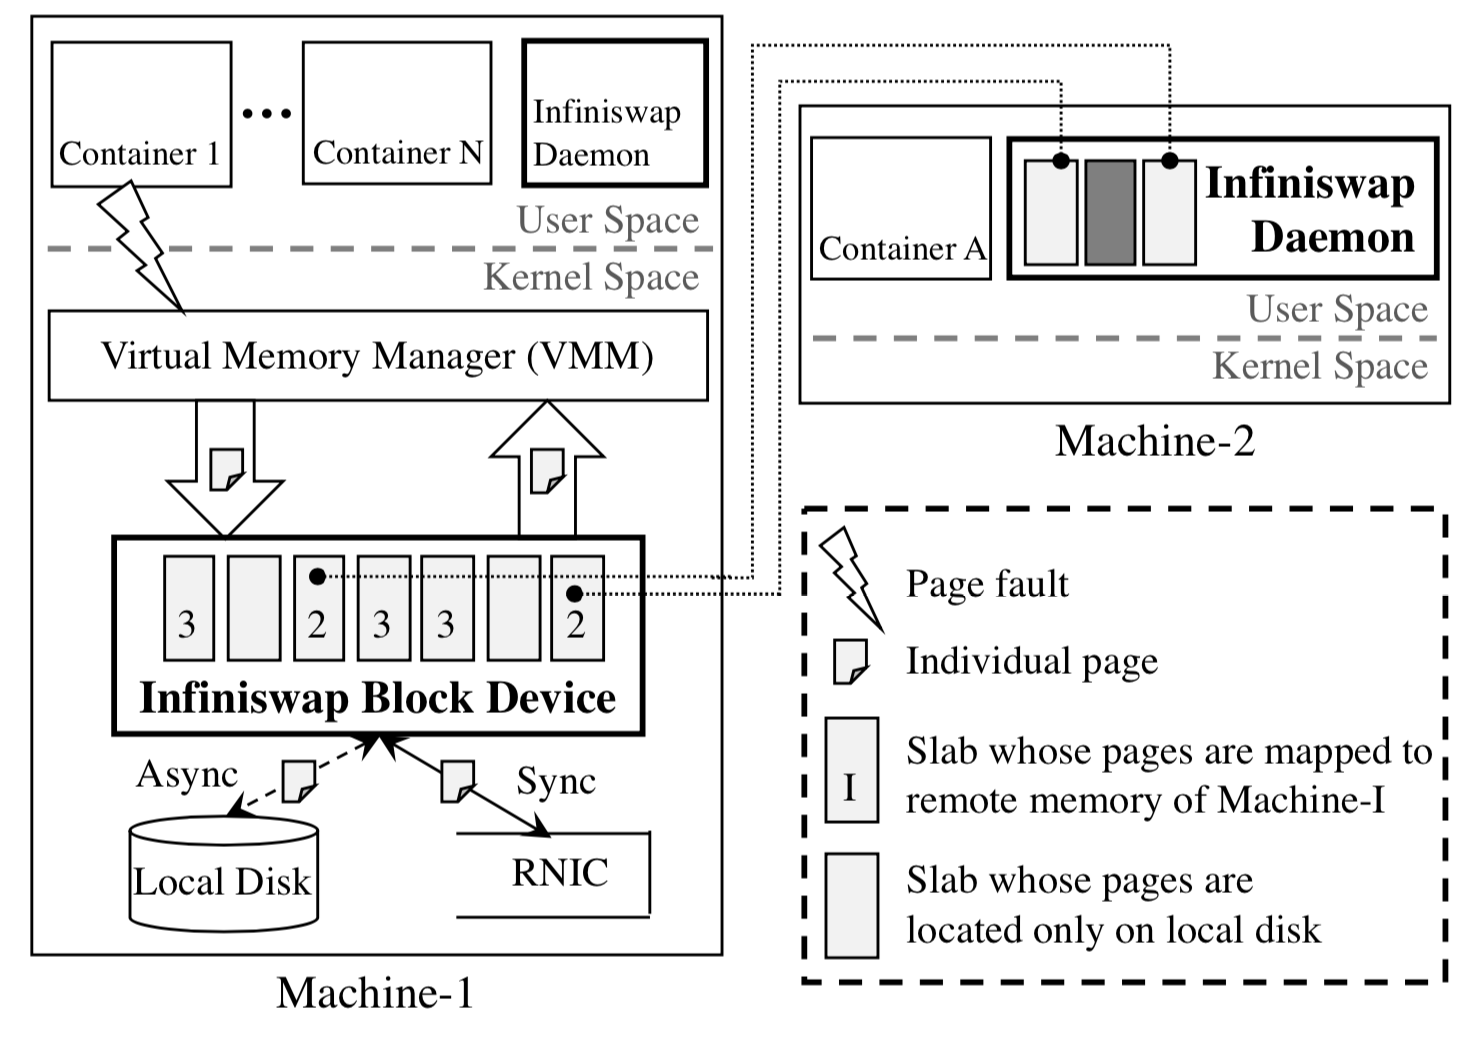
\includegraphics[scale=0.5]{Figures/memory/infiniswap_architecture.png}
\decoRule
\caption{INFINISWAP系统架构。\cite{gu2017efficient}}
\label{fig:infiniswap_architecture}
\end{figure}

\subsection{架构概述}
INFINISWAP包含了两个主要的组件——INFINISWAP块设备和INFINISWAP守护进程。
每台机器上都包含着这两个组件,因此每台机器的角色相同,从而实现了一个去中心化的系统(图~\ref{fig:infiniswap_architecture})。

\subsubsection{INFINISWAP块设备}
INFINISWAP块设备向虚拟内存管理器提供常规的块设备IO接口,让虚拟内存管理器将这个设备当成是一个交换分区。
当出现换页的时候,INFINISWAP块设备便可以透明地通过RDMA操作向其它机器中读取内存或写入内存。

INFINISWAP将每台机器上的内存地址空间划分成固定大小的大块(slab),大块是INFINISWAP内存映射和负载均衡的基本单位,它由很多内存页所组成。
以大块为单位进行内存映射处理的原因尽量减少远端机器上CPU的参与,减少对远端机器上应用程序的打扰,同时提升远程换页的速度。
当大块映射完毕之后,INFINISWAP块设备便可以通过RDMA读写操作来进行换页,换页的基本单位仍然是内存页,而不是大块。

\subsubsection{INFINISWAP守护进程}
INFINISWAP守护进程是运行在用户态的一个程序,仅仅参与控制层面(control plane)的活动。
它仅仅负责处理其它机器发过来的大块映射请求以及预先分配相应的内存空间。
真正的对数据层面(data plane)的操作则是通过RDMA请求然后由网卡去执行,并不会打扰目标机器的CPU。

\subsection{设计与实现}

\subsubsection{透明性和隔离性设计}
\paragraph{透明性}
INFINISWAP提供与传统块设备一样的接口和语义,应用程序不需要做任何修改便可以使用到更多的内存,它也不知道自己使用的是本地内存还是远程内存。
这样的透明性使得INFINISWAP系统具有很好的兼容性与通用性,能在现有的数据中心快速通入使用,不需要增加新的硬件。

\paragraph{隔离性}
INFINISWAP使用RDMA高速网络来传输内存页数据,不需要打扰远端CPU的执行。
对远程CPU的打扰主要在于大块的映射,但大块的大小是比内存页要大很多的,这样的一个设计也为了减少对远端机器CPU的打扰次数。

\subsubsection{容错性设计}
INFINISWAP对应用程序是透明的,应用程序认为远端机器上面的内存也是存在于本地的。
因此,INFINISWAP需要提供与应用程序只使用本地内存一样的语义,即当远端机器出现错误时,不能影响到本地应用的运行。

容错的方案是在进行RDMA远程换页的同时,异步地将内存也写入本地硬盘中做为备份。
由于写备份是异步的,并不在关键路径上,因此也不会对性能产生很大的影响。

实现这样的容错方案要处理一些边界问题,最重要的边界问题是处理\emph{read-after-write}的情况。
即当内存页已经写到远端的内存但还没有写入本地硬盘中,在这时候远端机器发生了崩溃。
如果在这同时应用程序又要读取这块内存页,块设备便需要从硬盘的写队列中读取内存页,然后返回给应用程序。

\begin{figure}
\centering
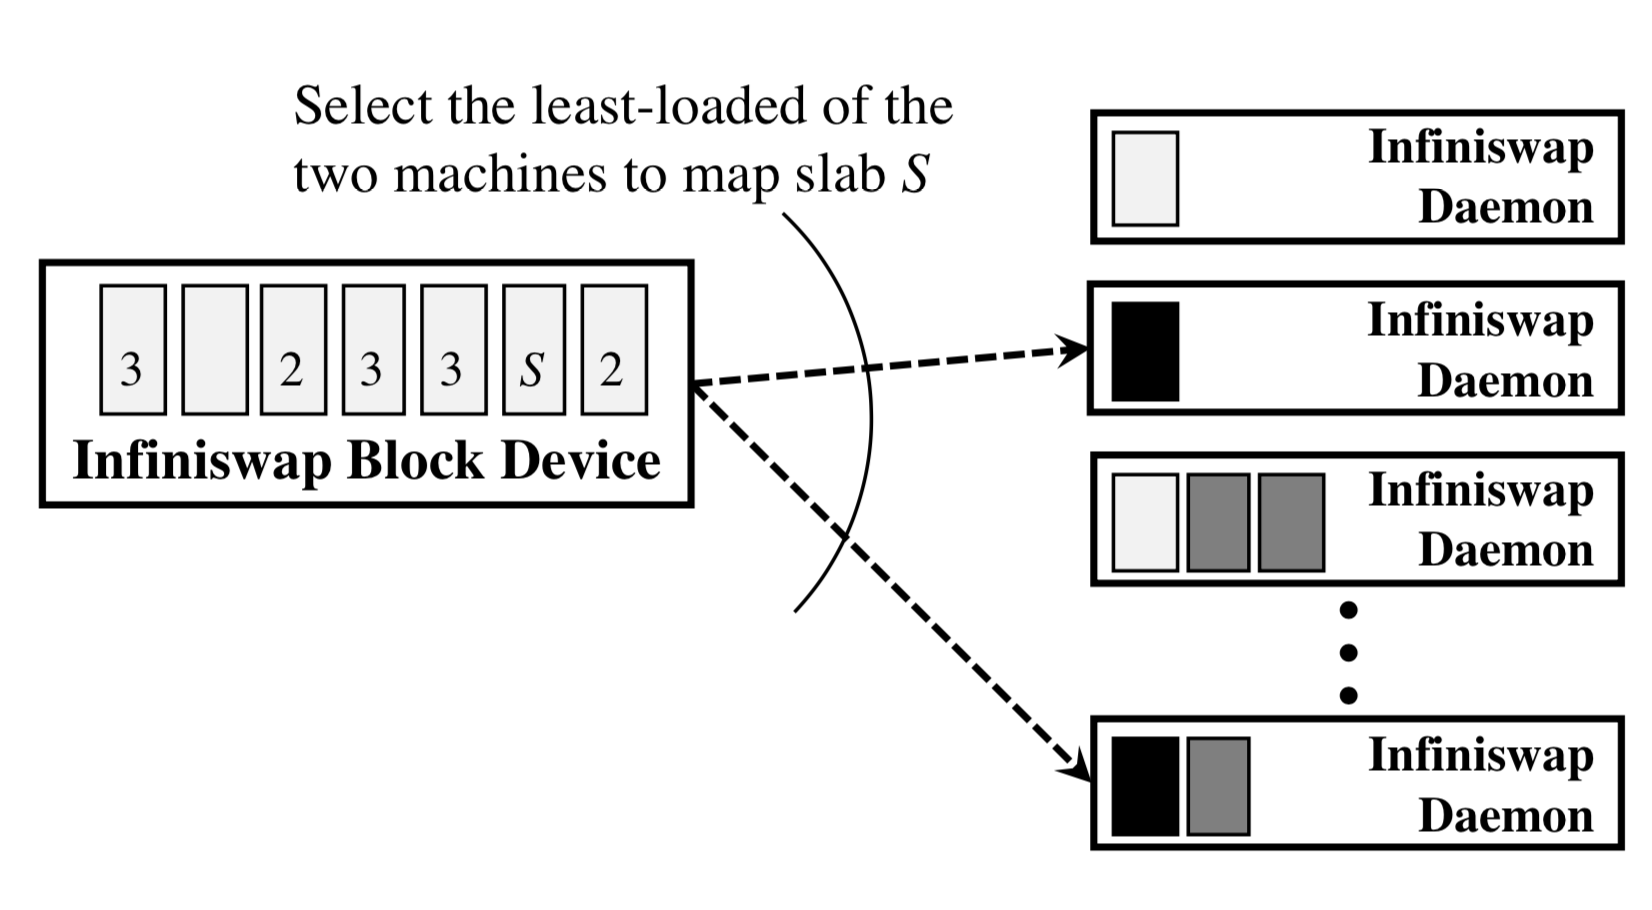
\includegraphics[scale=0.3]{Figures/memory/infiniswap_slab_mapping.png}
\decoRule
\caption{INFINISWAP块映射策略\cite{gu2017efficient}。}
\label{fig:infiniswap_slab_mapping}
\end{figure}

\begin{figure}
\centering
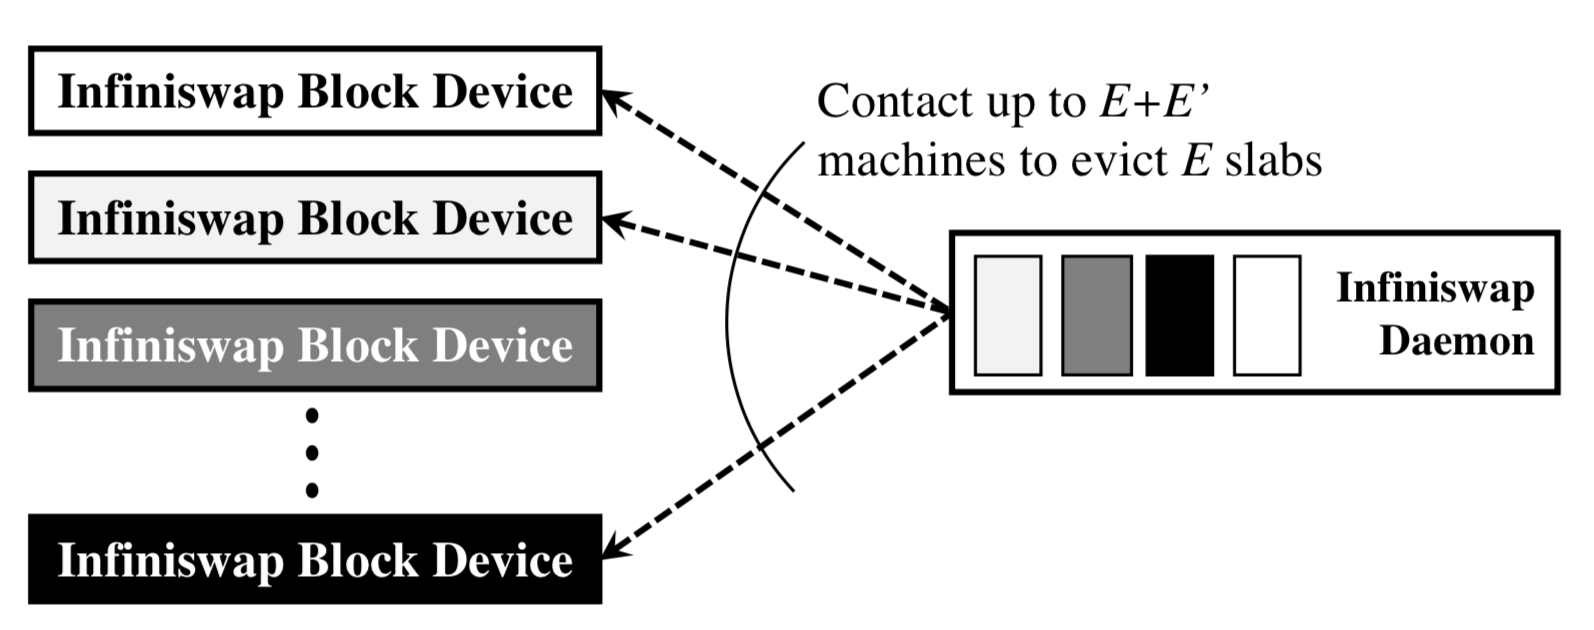
\includegraphics[scale=0.3]{Figures/memory/infiniswap_slab_eviction.png}
\decoRule
\caption{INFINISWAP块淘汰策略\cite{gu2017efficient}。}
\label{fig:infiniswap_slab_eviction}
\end{figure}

\subsubsection{可拓展性设计}
INFINISWAP并没有一个中心化的设计,避免由中央的协同器成为系统的瓶颈而导致系统不具有可拓展性。
去中心化的设计虽然能够使系统具备一定的可拓展性,但缺少中央协同器来收集全局的信息,这会带来很多问题。

其中关键的问题,如何制定好的大块映射策略来使得集群中每台机器的内存使用情况都趋于均衡。
INFINISWAP使用了\emph{power-of-choices}的技术来作为块映射以及块淘汰的策略。
比如\emph{power-of-two}的块映射策略,会先随机地选择两台远程机器,比较两台机器的内存使用情况,然后选择内存使用较少的一台机器作为目标机器来进行块映射。
类似地,块淘汰策略也是使用了\emph{power-of-choices}的方法。

\subsection{系统评测}
测试使用32台机器的集群,机器之间用56Gbps的Infiniswap网卡连接。
每台机器有2个NUMA节点和64GB的内存,每个NUMA节点有8个物理CPU,一共32个vCPU。

\begin{figure}
\centering
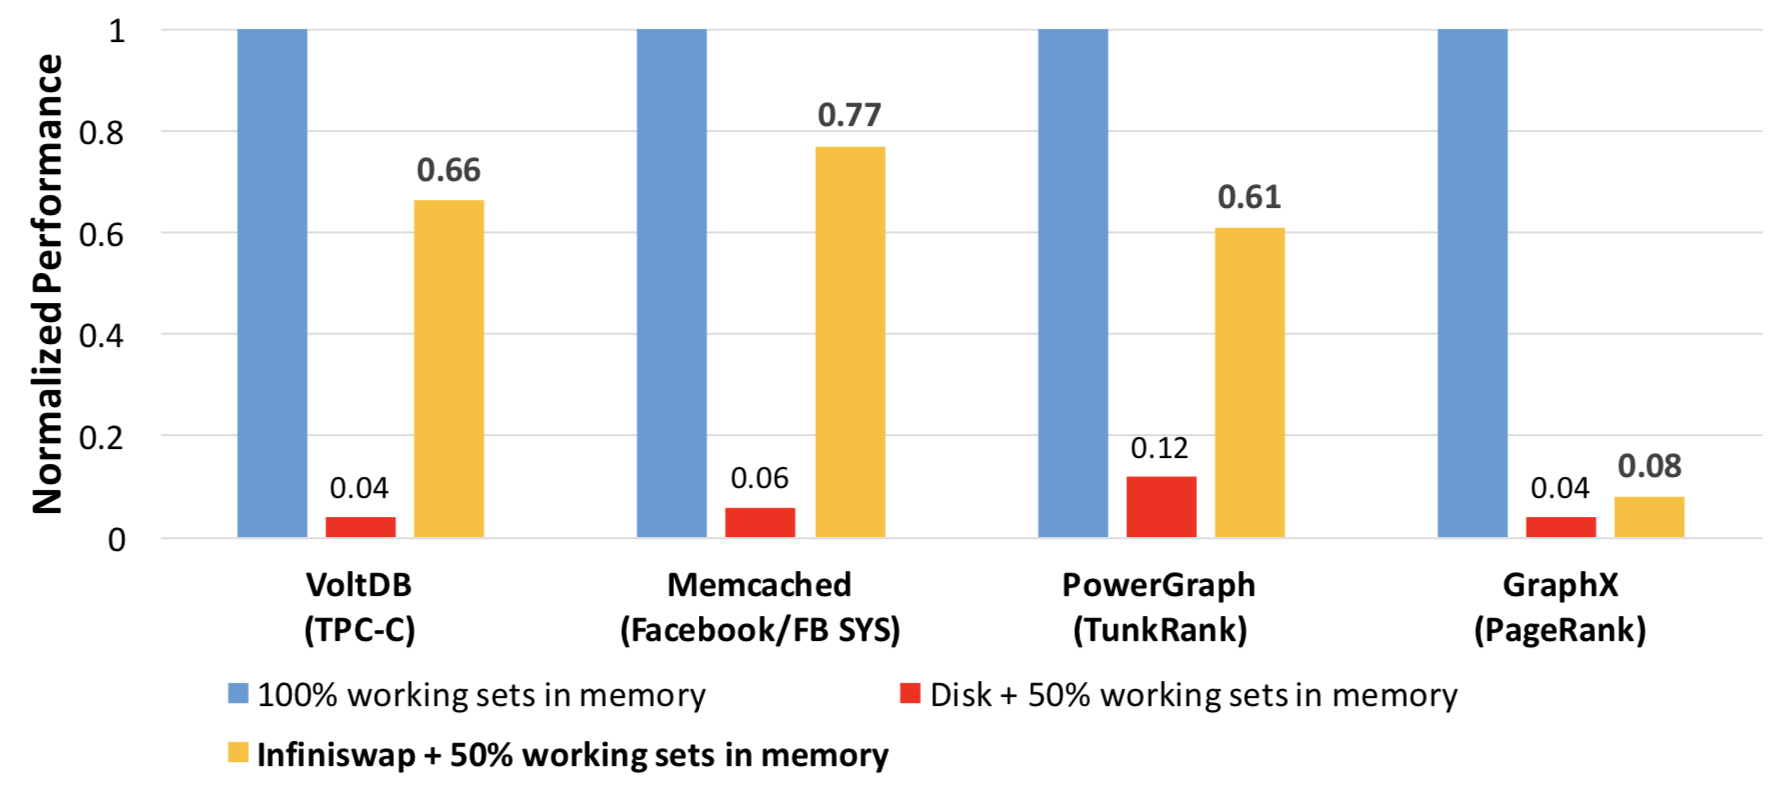
\includegraphics[scale=0.4]{Figures/memory/infiniswap_evaluation1.png}
\decoRule
\caption{应用程序的性能\cite{gu2017efficient}。}
\label{fig:infiniswap_evaluation1}
\end{figure}

\paragraph{应用程序的性能}
用于测试的应用程序有VoltDB、Memcached、PowerGraph和GraphX。
测试分别测了单机内存能满足应用程序100\%的内存需求、能满足应用程序50\%的内存需求和满足应用程序50\%的内存需求并使用INFINISWAP系统三种情况下应用程序的性能(图~\ref{fig:infiniswap_evaluation1})。
最终的测试结果表明,在单机内存只能满足应用程序50\%的内存需求时,使用INFINISWAP能将应用程序的性能提升2到16倍。

\paragraph{集群的内存使用情况}
测试创建了90个容器运行在集群上,每个容器使用不同的内存需求配置。
测试的结果显示集群的平均内存利用率从40.8\%提升到了60\%,提升了1.47倍。
而内存的不均衡现象也有所缓解(图~\ref{fig:infiniswap_evaluation2})。

\begin{figure}
\centering
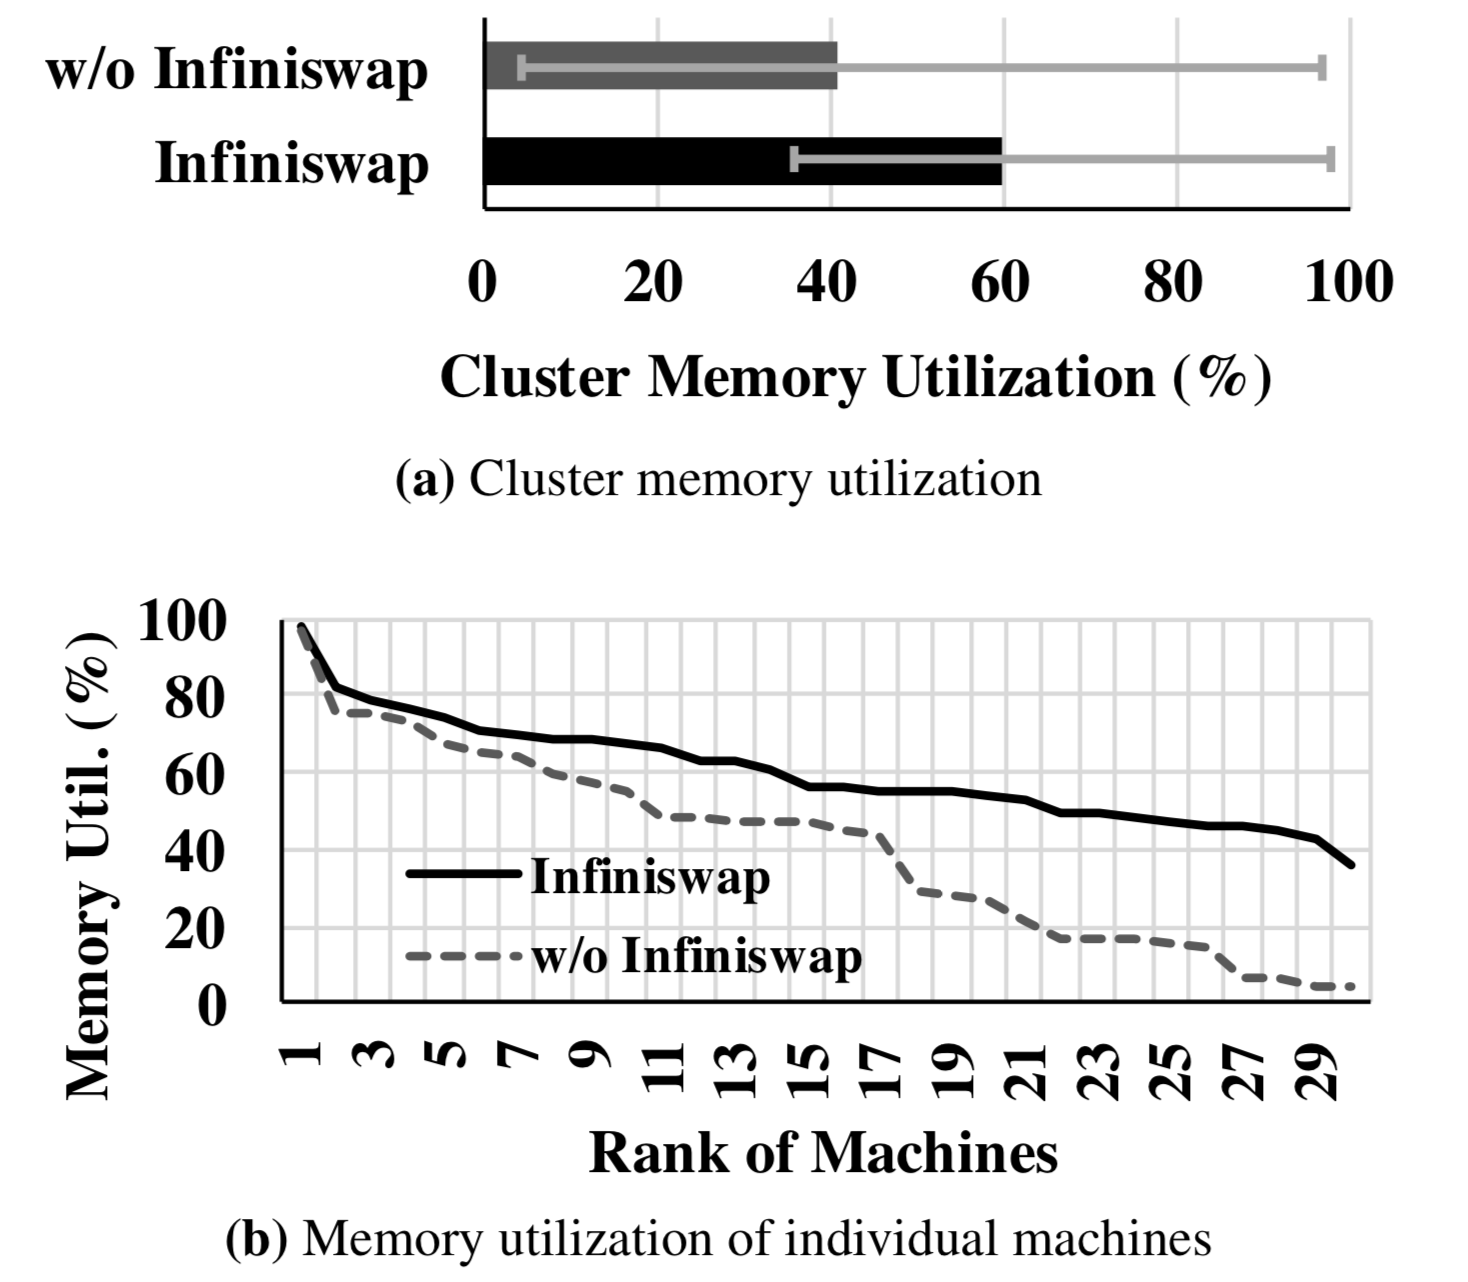
\includegraphics[scale=0.3]{Figures/memory/infiniswap_evaluation2.png}
\decoRule
\caption{集群的内存使用情况\cite{gu2017efficient}。}
\label{fig:infiniswap_evaluation2}
\end{figure}


%----------------------------------------------------------------------------------------
%	SECTION 4
%----------------------------------------------------------------------------------------

\section{本章小结}

本章介绍了内存分离的背景、研究现状和技术案例,说明了内存分离的重要性和可行性。
当下,内存分离技术正逐渐成为服务器架构的一种演变趋势,因为数据中心正迫切地想让资源能够更有效地利用。

实现内存分离有很多种技术方案,但无论哪种方案,都需要依靠网络来进行数据传输。
向前推动内存分离技术发展的重要技术动力是网络的发展。
虽然内存分离并不一定得要高速的网络才能实现,但越来越快的网络使得内存分离真正变得更加切实可行。

另外一方面,要打破传统的思维约束,使用革新方法去解决问题。
内存不足以及内存使用不均衡的根本原因是一体化服务器的架构,基于这样的架构去实现内存分离只是缓解了问题,并没有从根本上去解决。
在后面的章节中,我们将介绍LegoOS,看看如何从根本上去解决内存的相关问题。
